\section{Results}

\subsection{Training Model History}

\begin{figure}[htbp]
    \centering

    \begin{subfigure}[b]{0.48\textwidth}
        \centering
        \includegraphics[width=\textwidth]{figures/plots/loss_history.png}
        \caption{Changes in model loss over epochs}
        \label{fig:first}
    \end{subfigure}
    \hfill
    \begin{subfigure}[b]{0.48\textwidth}
        \centering
        \includegraphics[width=\textwidth]{figures/plots/accuracy_history.png}
        \caption{Changes in model accuracy over epochs}
        \label{fig:second}
    \end{subfigure}

    \caption{The above models show the progress of the models (a) loss and (b) accuracy. By looking at the separation between the training and validation curves, we can understand the model is not over fitting the training data.}
    \label{fig:side_by_side}
\end{figure}

\subsection{Base Model Results}

The confusion matrix is very important and efficient in showing the results of the algorithm against the test data. Figure~\ref{fig:acc_conf_matrix} shows the accuracy confusion matrix and how well the test went. The majority of misclassified results are false positives where the model assumed transit signals were eclipsing binaries. This is evident by the result of \textbf{(What percent?)}\% of eclipsing binaries being incorrectly classified. Comparatively, only \textbf{(What percent?)}\% of transits were misclassified. This shows the model prefers to call instances as transits in more cases than not. 

\begin{figure}
    \centering
    \includegraphics[width=0.5\linewidth]{figures/plots/real_confusion_matrix}
    \caption{The above plot is a simple 2x2 confusion matrix. The results show that the model comfortably classifies the true transits but is not able to make confident predictions for eclipsing binary cases.}
    \label{fig:acc_conf_matrix}
\end{figure}

Another pair of metrics we can use to see the quality of the model and its ability to classify instances is shown in Table~\ref{tab:metrics_table}. Accuracy has already been shown as of the confusion matrix above but the precision and recall explain the disparity much clearer. As the precision is very high we can conclude the model can comfortably classify transit light curves appropriately. It is the recall which raises the error as the value is very low. It tells the model misses a large chunk of eclipsing binaries. Thus the model prefers to default to transits over coming to an informed decision. 

\begin{table}[]
    \centering
    \begin{tabular}{c|c}
        Accuracy & 0.8637 \\ \hline
        Precision & 0.9236 \\ \hline
        Recall & 0.7956\\ \hline
        F1 Score & 0.8548\\ \hline
        ROC AUC & 0.9113
    \end{tabular}
    \caption{The above table shows the final metrics of the model. All scores are fine but for use on new data the results need to be improved to increase reliability.}
    \label{tab:metrics_table}
\end{table}

\subsection{Major Concern \textbf{Need better title}}

\begin{figure}
    \centering
    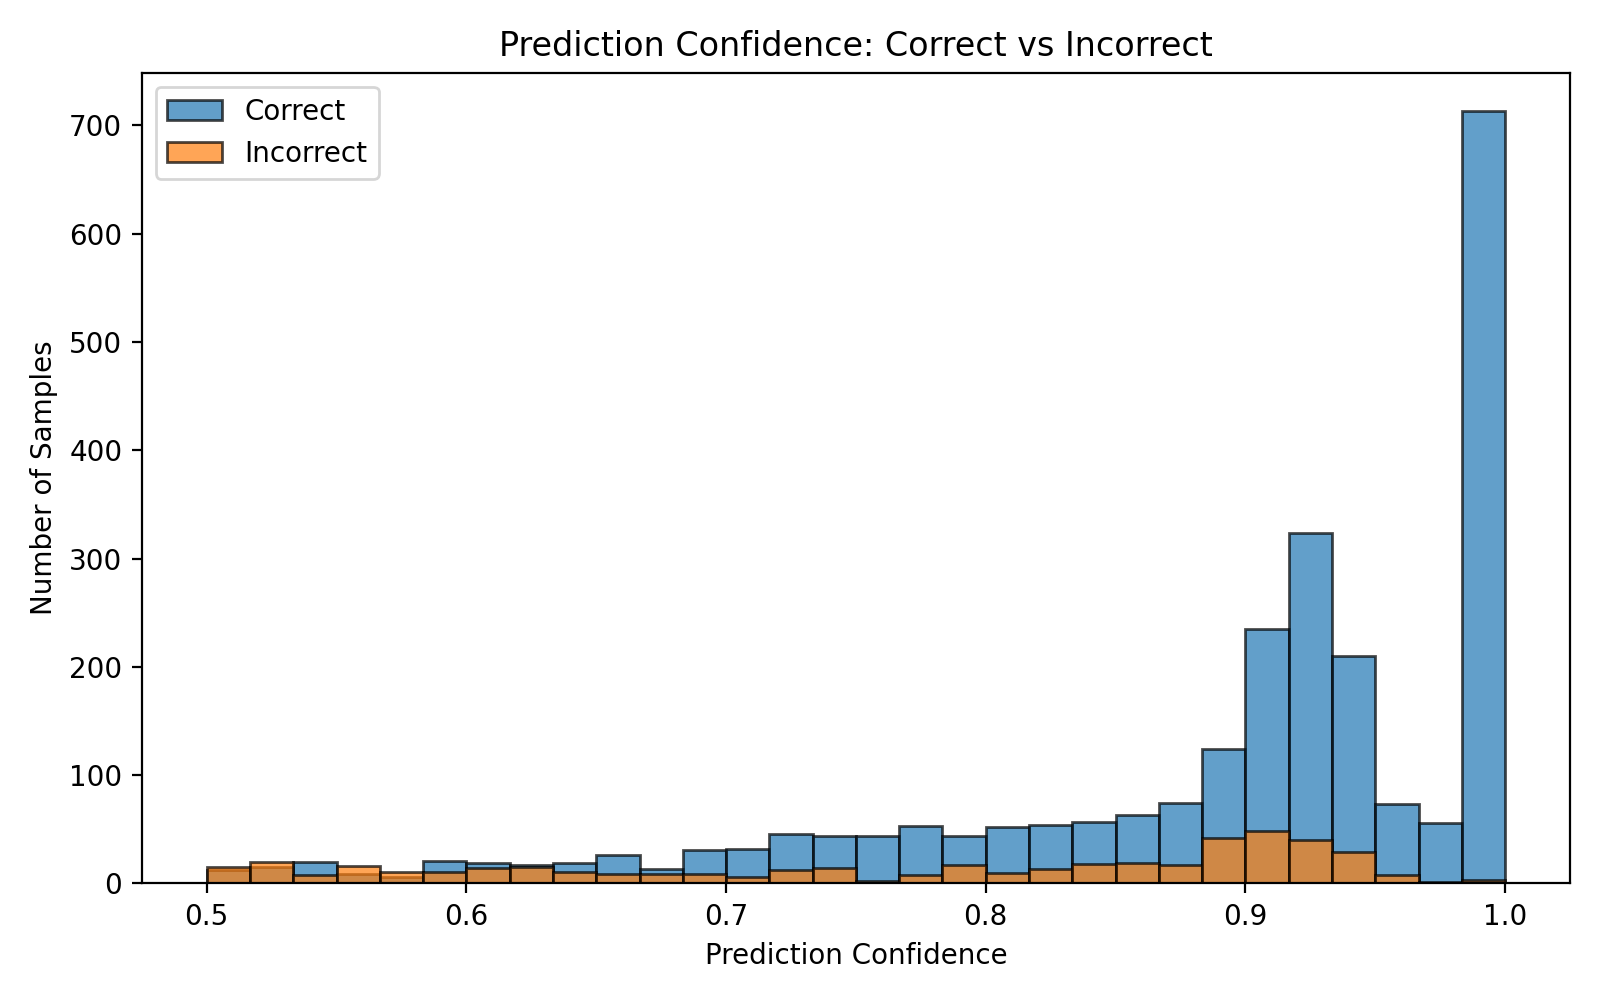
\includegraphics[width=0.5\linewidth]{figures/plots/confidence_correct_vs_incorrect.png}
    \caption{A histogram showing the spread of frequency of each confidence value the model returned. All correct classifications shown in \textbf{(Insert colour)} while incorrect classifications shown in \textbf{(Insert colour)}. An interesting bump in mistakes by the model is found in the \textbf{(What range? I think 0.8 to 0.9)}}
    \label{fig:conf_corr_vs_incorr_hist}
\end{figure}

Figure~\ref{fig:conf_corr_vs_incorr_hist} shows the distribution of all test instances by the models confidence in its classifications. A majority of classifications are correct with most falling with confidence of $0.8$ or greater. This makes sense when considering the metrics from Table~\ref{tab:metrics_table}. The focus in on the incorrect classifications as this gives info on the models mistakes. The incorrect bins sitting in the low range indicate typical errors in algorithms indicating where the model is unsure and likely guesses hoping to win the 50/50 chance. The focus is on the incorrect classifications with high confidence. Here the model was very sure of its decision but was incorrect which raises concerns as to why. 

One estimate is there is a correlation to the signal to noise ratio (SNR). In order to check this case we take the signal to noise ratio of each instance both from the \textit{Kepler} Archive and the simple equation using the transit depths. To analyse if this is the case, the false negatives which represent the misclassified eclipsing binaries need to be observed at different confidence ranges. As confidence can only sit between 0.5 (completely unsure) to 1.0 (extremely confident), the low range is set from $0.5$ to $0.7$, medium range from $0.7$ to $0.8$ and high for $0.8$ to $1.0$ \textbf{(Check these ranges for final publish}. 

\begin{figure}
    \centering
    \includegraphics[width=0.5\linewidth]{}
    \caption{Caption}
    \label{fig:placeholder}
\end{figure}